\IEEEPARstart{D}{uring} the last 30 years the CPU has evolved tremendously, increasing the instructions per second from 0.2 MIPS on the Intel 8088 in 1979\cite{reference:intel} to 177 730 MIPS on the Intel Core Extreme Edition i7-3960X in 2011 \cite{reference:inteli7}, while the memory performance has barely moved. Because of this gap, the memory access speed is acting as a bottleneck in the pipeline, where the CPU has to wait for the fetch operation to finish. This wait is shortened a bit by launching new instructions that were determined to be uncorrelated to the queried memory fetch, but it doesn't do that much difference on overall performance.

The invention of the virtual memory space allowed a memory hierarchy system to be implemented. This way, large, inexpensive, slow memory like RAM can be combined with small, fast, expensive memory onchip memory. The desired memory is "cached" in the onchip memory in blocks, and the process can be accelerated significantly by only having to access onchip memory instead of RAM. If memory that is to be referenced together has addresses that are close in virtual memory, the probablity of it already being cached increases. The probability of a cache hit depends heavily on cache size and the size of the memory block that is cached each time the memory manager needs to access the RAM. In addition to the onchip and offchip memory split, it is common to have both two and three levels of data cache on chip, with L1 cache being the highest level, lying closest to the processing core, often local to the core it services. While this makes the performance a lot better than with off chip memory alone, it doesn't do much for the cases where the memory address isn't cached. The processor is still waiting for accesses, and the limited size of the cache (the aforementioned Intel i7-processor features a 15MB L3 cache, which puts it at the top of the desktop-game). 

In an effort to reduce the wait associated with memory access on the offchip memory, the prefetcher attempts to determine the address of the memory that is to be accessed before it's actually needed. The prefetcher was first introduced on the Intel 8086, and monitors cache misses, attempting to detect access patterns in the form of indepentent, interweaved streams of addresses \cite{reference:8086}. A perfect prefetcher would assure that the processor always had the desired memory in cache at the right time, but as the physical and memory address space the prefetcher is granted has to be minimal for it to have any benefit at all, the success is equally limited. 
\\
\begin{figure}[h!]
	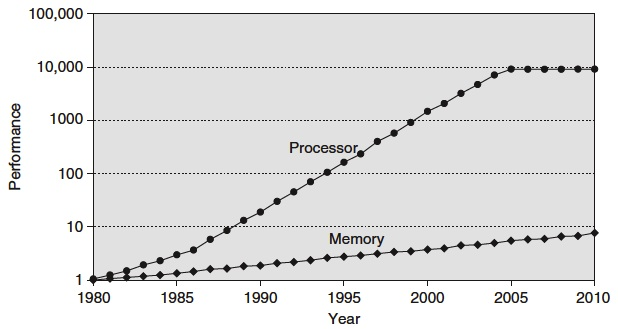
\includegraphics[width=3.5in]{graphics/CPUmemoryGap.jpg}
	\caption{Dette er ei tekning}
\end{figure}
\\
